\chapter{The principle neural architecture}

\section{Neurons perspective}

The formalization to be \textit{atoms} comes from the biological inspiration of exactly the biological neurons in human and species' brain. However, the mechanism and how they operate is a bit more interesting. 

For the biological more advanced equivalent, the brain consists of a very large number of highly connected elements, called \textit{neurons}. The simplified structure of such neuron consists of three components: the \textit{dendrite}, which is tree-like receptive network that carry signals (electrical) to the cell body; the \textit{cell body} effectively processes these signals, usually as sums and threshold response; and the \textit{axon}, a single long fibre that carries signal from the cell body to other neurons. The point of contact between an axon and a dendrite of another cell is called a synapse. The neural network, hence, is established by the synapses and various arrangements of the neuron. 

This configuration of biological neuron is particularly powerful. Not only that they can process information allowing someone to write this text, but also the fact that of billions or neuron, they parallelly work at the same time. Furthermore, the intricacy lies further ahead than the above formation - the entire structure is of too much complexity, for the brain itself. However, a principle can be seen - they are contained of \textit{building blocks} together, in which case is neuron. And \textbf{artificial networks} also take this approach. 

\begin{note}
From such, we can conclude that, we have to have some classification that requires the smallest component neuron to be the \textit{atoms} that everything else is formed upon.
\end{note}

One of the most fundamental thing of the structure of the \textit{neural network formalism}, hence, is the notion of a \textit{unit neuron}. Specifically, a neuron $x$ is defined, and designed to be a discrete operating unit on its own. The word \textit{operating} here means that it has all the facility requires for an input-output process - the most simple one includes the input receiver, the processing formulae, and the output transmitter. 

The neural network formalism is best expressed by the following principle. 

\begin{theorem}[The fundamental theorem of neural formalism]
    In the construction of an automated, artificial intelligence construct, the smallest singleton workable component must have the same size and dimension specified as the \textit{minimally defined neural structure}, $\mathfrak{N}(\mathcal{N},\mathcal{C})$. %\index{fundamental theorem of neural formalism}
\end{theorem}

We begin by examining the model of a typical neuron. Note that, this is the simplest one, but also is the fundamental block. We have the following. 

\begin{definition}[Neuron]
    Given the neural network formalism. Define a construct $x$. Then $x$ is called a \textbf{neuron} if it belongs component-wise to the class $\mathcal{N}$ of all neurons, which is minimally expressed by $\mathcal{N}(n_{i},n_{o},M(\dots))$, where $n_{i}$ is the input handler, $n_{o}$ is the output handler, and $M(\dots)$ is the internal system. %\index{classical neuron}
\end{definition}

From this, we then come up with the definition of the minimally defined neuron - the single most iteration of the above definition. 

\begin{definition}[Minimally defined neuron]
    Given the neural network formalism. Then, for $x\in \mathcal{N}$, we call a neuron \textbf{minimally defined} if it belongs to the class $\mathcal{N}_{0}\subset \mathcal{N}$ of $\mathcal{N}_{0}(n_{i}[\mathbf{w}],n_{o}[\mathbf{w}'],M(f,b))$ for $f:n_{i}[\mathbf{w}]\times b \to \mathcal{O}$ is the internal function of $M$. $\mathcal{O}$ is the domain of $n_{o}$ in which it receives the value, and in cases, there exists no $\mathbf{w}'$ configured for the output channel. %\index{minimally defined classical neuron}
\end{definition}

The notation $n_{i}[\mathbf{w}], n_{o}[\mathbf{w}']$ inherently indicate the notion of \textit{control} of the neuron on the two gate of input and output. More specifically, a given neuron, aside from the upper-level expression of $\mathcal{N}(\dots)$, can also be realized by its \textit{parameters}, or rather, its configuration of the neuron itself. By that, for $x \in \mathcal{N}$, the \textit{configuration parameters} for the minimally defined neuron can be taken in the form $\mathcal{C}(\mathbf{w}_{i}, \mathbf{w}_{o}, \mathbf{w}_{M})$, here we use instead the pairing notation. The letter $\mathbf{w}$ used here is historical by certain accounts: the original idea comes from the term \textbf{weight}, in which the neuron can conceptually influence the input, for example, the signal received or information received, by certain amount, either \textit{downplay} it or \textit{signify} it.

We clearly clarify the need for both $\mathcal{N}$ and $\mathcal{C}$ here. We know, that we want the neuron to be an \textit{operating unit}. This means that for it to be fully realized, it needs to also operate, and hence, to be 'observed'. Hence, you need both the description of the parameters which defines it - taken the interpretation where each parameter and configuration is one specific building block on its own, then the block of all those parameters form the shape of the neuron. Similarly, the \textit{operations} on such neuron assure the interaction and working mechanism of all those components together, inside the neuron, by itself. Hence, to fully, minimally express a minimalized neuron, you need to have both $\mathcal{N}$  and $\mathcal{C}$ as its minimality requirement. We then revise it to the following definition. 

\begin{definition}[Classical neuron class] \label{def:neuclass}
    Given the \textit{neural network formalism}. Then, we define a \textbf{neuron} $A$ to be \textit{minimally defined} if it is equivalent to any unit $x$ of the class $\mathfrak{N}_{m}(\mathcal{N}, \mathcal{C})$, called a \textit{neuron class}, where the 2-tuple expanded to $\mathcal{N}(n_{i}, n_{o}, M)$ and $\mathcal{C}(\mathbf{w}_{i}, \mathbf{w}_{o}, \mathbf{w}_{M})$. %\index{classical neuron class}
\end{definition}

\begin{figure}[!ht]
    \centering
    \resizebox{0.6\textwidth}{!}{%
    \begin{circuitikz}
    \tikzstyle{every node}=[font=\Large]
    
    % Manually place the label above the box
    \node at (29,7) {\Large $x\in\mathfrak{N}_{m}(\mathcal{N}, \mathcal{C})$};
    
    % Outer dashed box
    \draw[dashed] (21.75,6.25) rectangle (36.25,-1.25);
    
    % Inner boxes
    \draw (22,6) rectangle node {\Large $n_{i}[\mathbf{w}]$} (23.75,-1);
    \draw (36,6) rectangle node {\Large $n_{o}[\mathbf{w}']$} (34.25,-1);
    \draw (24,6) rectangle node {\Large $M(\dots)$} (34,-1);
    \end{circuitikz}
    }%
    \caption{Minimal neuron structure}
    \label{fig:lable}
\end{figure}

With this, we formalize the abstract neuron into two descriptions. Note that, however, the \textit{minimally defined} neuron has a parameterized exposure protocol to the construction. In practice, for any neuron $a \in \mathfrak{N}$, the tuple $(\mathcal{N}, \mathcal{C})$ can be different, not to say complex. One of the strong points of this construction of the neural class is that it is \textit{recursive}. The following proposition might help aid in understanding why it is recursive.

\begin{proposition}[Compound construction]
    An abstract neuron $A$  can be dissected into three most important compartments $(\mathrm{I},\mathrm{O},M)$, where $\mathrm{I},\mathrm{O}$ is respectively the in-out interface. Hence, a cluster of neurons $\{A_{i}\}_{i \leq n}$ for such $\lvert \{ A_{i} \} \rvert \geq 3$ can be compartmentalized into a new neuron unit, that is, $\{ A_{i} \}\in \mathfrak{N}$, if and only if $\lvert \{ A_{i} \} \rvert \geq 3$. 
\end{proposition}

\begin{proof}
    This mostly comes of as definition $(2.1)$. Notice that for any structure of a neuron to be minimally defined, the tuple $\mathcal{N}$ must minimally contain $(n_{i},n_{o},M)$. We want them to be discretely defined, then a cluster of neuron will have to have at least one neuron such that to satisfy the requirement of the 3-tuple component. If $n=\lvert \{ A_{i} \} \rvert=1$, it reduces to a singular neuron; for $n=2$, at least one compartment do not have any component, hence minimally we need 3 neurons to effectively be arranged as a neuron unit. This can be illustrated using \ref{fig:lalala}.
\end{proof}

\begin{figure}
    \centering
    \resizebox{0.6\textwidth}{!}
    {
\tikzset{every picture/.style={line width=0.75pt}} %set default line width to 0.75pt        

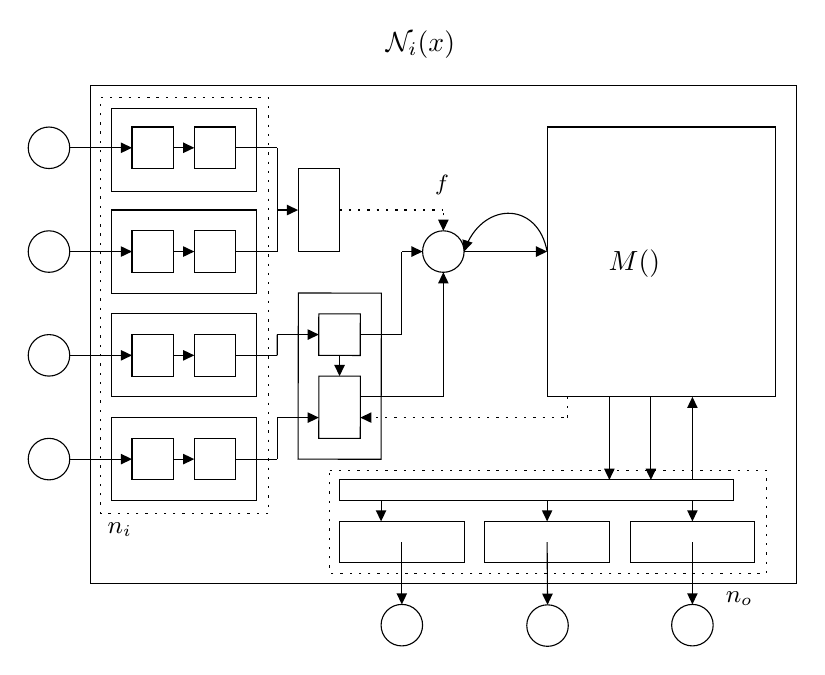
\begin{tikzpicture}[x=0.75pt,y=0.75pt,yscale=-1,xscale=1]
%uncomment if require: \path (0,439); %set diagram left start at 0, and has height of 439

%Shape: Rectangle [id:dp11325550993005518] 
\draw   (100,101) -- (170,101) -- (170,141) -- (100,141) -- cycle ;
%Shape: Rectangle [id:dp0871043429951639] 
\draw   (210,300) -- (270,300) -- (270,320) -- (210,320) -- cycle ;
%Shape: Rectangle [id:dp6243572067188583] 
\draw   (100,250) -- (170,250) -- (170,290) -- (100,290) -- cycle ;
%Shape: Rectangle [id:dp5814395527377063] 
\draw   (100,200) -- (170,200) -- (170,240) -- (100,240) -- cycle ;
%Shape: Rectangle [id:dp8753477258371138] 
\draw   (100,150) -- (170,150) -- (170,190) -- (100,190) -- cycle ;
%Shape: Rectangle [id:dp5798677682795597] 
\draw   (230.15,190.04) -- (230,270.08) -- (190,270) -- (190.15,189.96) -- cycle ;
%Shape: Rectangle [id:dp24707649617836847] 
\draw   (190,130) -- (210,130) -- (210,170) -- (190,170) -- cycle ;
%Shape: Rectangle [id:dp33716600057650536] 
\draw   (350,300) -- (410,300) -- (410,320) -- (350,320) -- cycle ;
%Shape: Rectangle [id:dp9055416056676429] 
\draw   (280,300) -- (340,300) -- (340,320) -- (280,320) -- cycle ;
%Shape: Rectangle [id:dp13764882951656032] 
\draw   (220,200.04) -- (219.96,220.06) -- (199.96,220.02) -- (200,200) -- cycle ;
%Shape: Rectangle [id:dp27863186768492065] 
\draw   (220.04,230.04) -- (219.98,260.02) -- (199.98,259.98) -- (200.04,230) -- cycle ;
%Shape: Rectangle [id:dp5553865711579786] 
\draw   (110,160) -- (130,160) -- (130,180) -- (110,180) -- cycle ;
%Shape: Rectangle [id:dp9842747920805606] 
\draw   (140,160) -- (160,160) -- (160,180) -- (140,180) -- cycle ;
%Shape: Rectangle [id:dp11391650551903476] 
\draw   (110,260) -- (130,260) -- (130,280) -- (110,280) -- cycle ;
%Shape: Rectangle [id:dp09942914368133748] 
\draw   (140,260) -- (160,260) -- (160,280) -- (140,280) -- cycle ;
%Shape: Rectangle [id:dp6297511200807524] 
\draw   (110,210) -- (130,210) -- (130,230) -- (110,230) -- cycle ;
%Shape: Rectangle [id:dp9307891959891459] 
\draw   (140,210) -- (160,210) -- (160,230) -- (140,230) -- cycle ;
%Shape: Rectangle [id:dp8446667441818969] 
\draw   (110,110) -- (130,110) -- (130,130) -- (110,130) -- cycle ;
%Shape: Rectangle [id:dp7846804351453478] 
\draw   (140,110) -- (160,110) -- (160,130) -- (140,130) -- cycle ;
%Straight Lines [id:da5110600464617441] 
\draw    (80,170) -- (107,170) ;
\draw [shift={(110,170)}, rotate = 180] [fill={rgb, 255:red, 0; green, 0; blue, 0 }  ][line width=0.08]  [draw opacity=0] (5.36,-2.57) -- (0,0) -- (5.36,2.57) -- cycle    ;
%Straight Lines [id:da5422700604803716] 
\draw    (80,120) -- (107,120) ;
\draw [shift={(110,120)}, rotate = 180] [fill={rgb, 255:red, 0; green, 0; blue, 0 }  ][line width=0.08]  [draw opacity=0] (5.36,-2.57) -- (0,0) -- (5.36,2.57) -- cycle    ;
%Shape: Rectangle [id:dp9313490804874551] 
\draw   (90,90) -- (430,90) -- (430,330) -- (90,330) -- cycle ;
%Straight Lines [id:da9105070856971889] 
\draw    (80,220) -- (107,220) ;
\draw [shift={(110,220)}, rotate = 180] [fill={rgb, 255:red, 0; green, 0; blue, 0 }  ][line width=0.08]  [draw opacity=0] (5.36,-2.57) -- (0,0) -- (5.36,2.57) -- cycle    ;
%Straight Lines [id:da6609395816932571] 
\draw    (80,270) -- (107,270) ;
\draw [shift={(110,270)}, rotate = 180] [fill={rgb, 255:red, 0; green, 0; blue, 0 }  ][line width=0.08]  [draw opacity=0] (5.36,-2.57) -- (0,0) -- (5.36,2.57) -- cycle    ;
%Straight Lines [id:da0032511945053963487] 
\draw    (130,270) -- (137,270) ;
\draw [shift={(140,270)}, rotate = 180] [fill={rgb, 255:red, 0; green, 0; blue, 0 }  ][line width=0.08]  [draw opacity=0] (5.36,-2.57) -- (0,0) -- (5.36,2.57) -- cycle    ;
%Straight Lines [id:da913878359208306] 
\draw    (130,220) -- (137,220) ;
\draw [shift={(140,220)}, rotate = 180] [fill={rgb, 255:red, 0; green, 0; blue, 0 }  ][line width=0.08]  [draw opacity=0] (5.36,-2.57) -- (0,0) -- (5.36,2.57) -- cycle    ;
%Straight Lines [id:da29849706207756643] 
\draw    (130,170) -- (137,170) ;
\draw [shift={(140,170)}, rotate = 180] [fill={rgb, 255:red, 0; green, 0; blue, 0 }  ][line width=0.08]  [draw opacity=0] (5.36,-2.57) -- (0,0) -- (5.36,2.57) -- cycle    ;
%Straight Lines [id:da5988492285356528] 
\draw    (130,120) -- (137,120) ;
\draw [shift={(140,120)}, rotate = 180] [fill={rgb, 255:red, 0; green, 0; blue, 0 }  ][line width=0.08]  [draw opacity=0] (5.36,-2.57) -- (0,0) -- (5.36,2.57) -- cycle    ;
%Shape: Rectangle [id:dp06329604948993794] 
\draw   (310,110) -- (420,110) -- (420,240) -- (310,240) -- cycle ;
%Flowchart: Connector [id:dp8332863887530595] 
\draw   (250,170) .. controls (250,164.48) and (254.48,160) .. (260,160) .. controls (265.52,160) and (270,164.48) .. (270,170) .. controls (270,175.52) and (265.52,180) .. (260,180) .. controls (254.48,180) and (250,175.52) .. (250,170) -- cycle ;
%Straight Lines [id:da12612212040876503] 
\draw    (160,120) -- (180,120) ;
%Straight Lines [id:da31914662032691554] 
\draw    (180,120) -- (180,150) ;
%Straight Lines [id:da9795534822739309] 
\draw    (180,150) -- (187,150) ;
\draw [shift={(190,150)}, rotate = 180] [fill={rgb, 255:red, 0; green, 0; blue, 0 }  ][line width=0.08]  [draw opacity=0] (5.36,-2.57) -- (0,0) -- (5.36,2.57) -- cycle    ;
%Straight Lines [id:da6816623316052335] 
\draw    (180,150) -- (180,170) ;
%Straight Lines [id:da10214644502871861] 
\draw    (160,170) -- (180,170) ;
%Straight Lines [id:da2333042550366453] 
\draw    (210,220) -- (210,227) ;
\draw [shift={(210,230)}, rotate = 270] [fill={rgb, 255:red, 0; green, 0; blue, 0 }  ][line width=0.08]  [draw opacity=0] (5.36,-2.57) -- (0,0) -- (5.36,2.57) -- cycle    ;
%Straight Lines [id:da6207516705964704] 
\draw    (160,220) -- (180,220) ;
%Straight Lines [id:da8944570569529915] 
\draw    (179.96,220.02) -- (180,210) ;
%Straight Lines [id:da8214897304050846] 
\draw    (180,210) -- (197,210) ;
\draw [shift={(200,210)}, rotate = 180] [fill={rgb, 255:red, 0; green, 0; blue, 0 }  ][line width=0.08]  [draw opacity=0] (5.36,-2.57) -- (0,0) -- (5.36,2.57) -- cycle    ;
%Straight Lines [id:da05957407818008731] 
\draw    (160,270) -- (180,270) ;
%Straight Lines [id:da49398447141544] 
\draw    (180,270) -- (180,250) ;
%Straight Lines [id:da711469323627808] 
\draw    (180,250) -- (197,250) ;
\draw [shift={(200,250)}, rotate = 180] [fill={rgb, 255:red, 0; green, 0; blue, 0 }  ][line width=0.08]  [draw opacity=0] (5.36,-2.57) -- (0,0) -- (5.36,2.57) -- cycle    ;
%Shape: Rectangle [id:dp7948056890037245] 
\draw   (210,280) -- (400,280) -- (400,290) -- (210,290) -- cycle ;
%Straight Lines [id:da8505206798497769] 
\draw  [dash pattern={on 0.84pt off 2.51pt}]  (210,150) -- (260,150) ;
%Straight Lines [id:da9415887071519273] 
\draw  [dash pattern={on 0.84pt off 2.51pt}]  (223,250) -- (320,250) ;
\draw [shift={(220,250)}, rotate = 0] [fill={rgb, 255:red, 0; green, 0; blue, 0 }  ][line width=0.08]  [draw opacity=0] (5.36,-2.57) -- (0,0) -- (5.36,2.57) -- cycle    ;
%Straight Lines [id:da837491588082458] 
\draw    (220,210) -- (240,210) ;
%Straight Lines [id:da06293690723018686] 
\draw    (240,210) -- (240,170) ;
%Straight Lines [id:da7200921856093905] 
\draw    (240,170) -- (247,170) ;
\draw [shift={(250,170)}, rotate = 180] [fill={rgb, 255:red, 0; green, 0; blue, 0 }  ][line width=0.08]  [draw opacity=0] (5.36,-2.57) -- (0,0) -- (5.36,2.57) -- cycle    ;
%Straight Lines [id:da7500647994920802] 
\draw    (220,240) -- (260,240) ;
%Straight Lines [id:da039805258182520564] 
\draw    (260,240) -- (260,183) ;
\draw [shift={(260,180)}, rotate = 90] [fill={rgb, 255:red, 0; green, 0; blue, 0 }  ][line width=0.08]  [draw opacity=0] (5.36,-2.57) -- (0,0) -- (5.36,2.57) -- cycle    ;
%Straight Lines [id:da23764718408033914] 
\draw  [dash pattern={on 0.84pt off 2.51pt}]  (320,240) -- (320,250) ;
%Straight Lines [id:da4687498151820695] 
\draw  [dash pattern={on 0.84pt off 2.51pt}]  (260,157) -- (260,150) ;
\draw [shift={(260,160)}, rotate = 270] [fill={rgb, 255:red, 0; green, 0; blue, 0 }  ][line width=0.08]  [draw opacity=0] (5.36,-2.57) -- (0,0) -- (5.36,2.57) -- cycle    ;
%Straight Lines [id:da24885446056205818] 
\draw    (340,277) -- (340,240) ;
\draw [shift={(340,280)}, rotate = 270] [fill={rgb, 255:red, 0; green, 0; blue, 0 }  ][line width=0.08]  [draw opacity=0] (5.36,-2.57) -- (0,0) -- (5.36,2.57) -- cycle    ;
%Straight Lines [id:da9151151693612134] 
\draw    (360,277) -- (360,240) ;
\draw [shift={(360,280)}, rotate = 270] [fill={rgb, 255:red, 0; green, 0; blue, 0 }  ][line width=0.08]  [draw opacity=0] (5.36,-2.57) -- (0,0) -- (5.36,2.57) -- cycle    ;
%Straight Lines [id:da1416977299387372] 
\draw    (380,280) -- (380,243) ;
\draw [shift={(380,240)}, rotate = 90] [fill={rgb, 255:red, 0; green, 0; blue, 0 }  ][line width=0.08]  [draw opacity=0] (5.36,-2.57) -- (0,0) -- (5.36,2.57) -- cycle    ;
%Straight Lines [id:da36064488959539687] 
\draw    (230,297) -- (230,290) ;
\draw [shift={(230,300)}, rotate = 270] [fill={rgb, 255:red, 0; green, 0; blue, 0 }  ][line width=0.08]  [draw opacity=0] (5.36,-2.57) -- (0,0) -- (5.36,2.57) -- cycle    ;
%Straight Lines [id:da06458094043292584] 
\draw    (310,297) -- (310,290) ;
\draw [shift={(310,300)}, rotate = 270] [fill={rgb, 255:red, 0; green, 0; blue, 0 }  ][line width=0.08]  [draw opacity=0] (5.36,-2.57) -- (0,0) -- (5.36,2.57) -- cycle    ;
%Straight Lines [id:da5371693206109713] 
\draw    (380,297) -- (380,290) ;
\draw [shift={(380,300)}, rotate = 270] [fill={rgb, 255:red, 0; green, 0; blue, 0 }  ][line width=0.08]  [draw opacity=0] (5.36,-2.57) -- (0,0) -- (5.36,2.57) -- cycle    ;
%Straight Lines [id:da14487306050826643] 
\draw    (307,170) -- (270,170) ;
\draw [shift={(310,170)}, rotate = 180] [fill={rgb, 255:red, 0; green, 0; blue, 0 }  ][line width=0.08]  [draw opacity=0] (5.36,-2.57) -- (0,0) -- (5.36,2.57) -- cycle    ;
%Curve Lines [id:da6990479809556309] 
\draw    (271.17,166.88) .. controls (280.24,145.78) and (305.61,146.13) .. (310,170) ;
\draw [shift={(270,170)}, rotate = 287.86] [fill={rgb, 255:red, 0; green, 0; blue, 0 }  ][line width=0.08]  [draw opacity=0] (5.36,-2.57) -- (0,0) -- (5.36,2.57) -- cycle    ;
%Straight Lines [id:da8358677637506173] 
\draw    (240,310) -- (240,337) ;
\draw [shift={(240,340)}, rotate = 270] [fill={rgb, 255:red, 0; green, 0; blue, 0 }  ][line width=0.08]  [draw opacity=0] (5.36,-2.57) -- (0,0) -- (5.36,2.57) -- cycle    ;
%Straight Lines [id:da244617897188945] 
\draw    (310,310) -- (310.18,337.2) ;
\draw [shift={(310.2,340.2)}, rotate = 269.62] [fill={rgb, 255:red, 0; green, 0; blue, 0 }  ][line width=0.08]  [draw opacity=0] (5.36,-2.57) -- (0,0) -- (5.36,2.57) -- cycle    ;
%Straight Lines [id:da5771038762158682] 
\draw    (380,310) -- (380,337) ;
\draw [shift={(380,340)}, rotate = 270] [fill={rgb, 255:red, 0; green, 0; blue, 0 }  ][line width=0.08]  [draw opacity=0] (5.36,-2.57) -- (0,0) -- (5.36,2.57) -- cycle    ;
%Shape: Rectangle [id:dp624674318079391] 
\draw  [dash pattern={on 0.84pt off 2.51pt}] (205.2,275.4) -- (415.8,275.4) -- (415.8,325) -- (205.2,325) -- cycle ;
%Shape: Rectangle [id:dp9005135043880514] 
\draw  [dash pattern={on 0.84pt off 2.51pt}] (95,95.8) -- (175.8,95.8) -- (175.8,296.2) -- (95,296.2) -- cycle ;
%Flowchart: Connector [id:dp5628657474616012] 
\draw   (60,120) .. controls (60,114.48) and (64.48,110) .. (70,110) .. controls (75.52,110) and (80,114.48) .. (80,120) .. controls (80,125.52) and (75.52,130) .. (70,130) .. controls (64.48,130) and (60,125.52) .. (60,120) -- cycle ;
%Flowchart: Connector [id:dp8272773414381507] 
\draw   (60,170) .. controls (60,164.48) and (64.48,160) .. (70,160) .. controls (75.52,160) and (80,164.48) .. (80,170) .. controls (80,175.52) and (75.52,180) .. (70,180) .. controls (64.48,180) and (60,175.52) .. (60,170) -- cycle ;
%Flowchart: Connector [id:dp28635133100043864] 
\draw   (60,220) .. controls (60,214.48) and (64.48,210) .. (70,210) .. controls (75.52,210) and (80,214.48) .. (80,220) .. controls (80,225.52) and (75.52,230) .. (70,230) .. controls (64.48,230) and (60,225.52) .. (60,220) -- cycle ;
%Flowchart: Connector [id:dp25327538239021874] 
\draw   (60,270) .. controls (60,264.48) and (64.48,260) .. (70,260) .. controls (75.52,260) and (80,264.48) .. (80,270) .. controls (80,275.52) and (75.52,280) .. (70,280) .. controls (64.48,280) and (60,275.52) .. (60,270) -- cycle ;
%Flowchart: Connector [id:dp12682149272136733] 
\draw   (230,350) .. controls (230,344.48) and (234.48,340) .. (240,340) .. controls (245.52,340) and (250,344.48) .. (250,350) .. controls (250,355.52) and (245.52,360) .. (240,360) .. controls (234.48,360) and (230,355.52) .. (230,350) -- cycle ;
%Flowchart: Connector [id:dp6810137569820218] 
\draw   (300.2,350.2) .. controls (300.2,344.68) and (304.68,340.2) .. (310.2,340.2) .. controls (315.72,340.2) and (320.2,344.68) .. (320.2,350.2) .. controls (320.2,355.72) and (315.72,360.2) .. (310.2,360.2) .. controls (304.68,360.2) and (300.2,355.72) .. (300.2,350.2) -- cycle ;
%Flowchart: Connector [id:dp01731761461300274] 
\draw   (370,350) .. controls (370,344.48) and (374.48,340) .. (380,340) .. controls (385.52,340) and (390,344.48) .. (390,350) .. controls (390,355.52) and (385.52,360) .. (380,360) .. controls (374.48,360) and (370,355.52) .. (370,350) -- cycle ;

% Text Node
\draw (231,62.4) node [anchor=north west][inner sep=0.75pt]    {$\mathcal{N}_{i}( x)$};
% Text Node
\draw (338.4,167.8) node [anchor=north west][inner sep=0.75pt]    {$M( \dotsc )$};
% Text Node
\draw (394.8,332.6) node [anchor=north west][inner sep=0.75pt]  [font=\small]  {$n_{o}$};
% Text Node
\draw (97,299.6) node [anchor=north west][inner sep=0.75pt]  [font=\small]  {$n_{i}$};
% Text Node
\draw (254.8,131.8) node [anchor=north west][inner sep=0.75pt]  [font=\footnotesize]  {$f$};
\end{tikzpicture}
    }
    \caption{The compound structure construction. The same component can be seen, for $n_i,n_o$ and $M$. Multiple consecutive components construct some components, and further outward. Also, we also reflect the complexity of $\mathcal{C}$ for a given architecture.}
    \label{fig:lalala}
\end{figure}

Hence, we can recursively define neuron, either going up or down, if they satisfy such condition. However, usually, we will only go up, as we will have to define in detail the set $\{ A_{M,i} \}$ of all possible \textit{minimally defined} neuron. \footnote{At this point, I am considering using \textit{group theory} to aid such set compartment.}

There are several assumptions and properties accompanied by this type of neuron structure that we would like to note.
\begin{enumerate}
    \item This neuron structure works \textit{sequentially}. A minimally defined neuron, such as in a practical setting, will have $\mathcal{C}$ to support sequential operation. What this means is present in the definition of the minimal neuron, such that $\mathcal{C} = (\mathbf{w}_{i}, \mathbf{w}_{o}, \mathbf{w}_{M})$, and the operation follows $i \to M \to o$ for an input-process-output session.
    
    \item By extension of the point above, the neuron order in a cluster will also be \textit{fixed}. Usually, this follows a single dimension, or, for example, if there exists a singular span directional vector $\vec{dr}$ that indicates the direction of operation in the cluster.
    
    \item We suppose the \textit{independence} of any components inside a neuron.
    
    \item The neuron is expressed in a \textit{parameterized manner}. That is, the behaviour of the neuron can be expressed, controlled, and designed by modifying and constructing a set of non-realized parameters. If this set of parameters is finite, we say that it is \textit{closed parameterization}. If not—i.e., there can be infinitely many parameters—we call it \textit{open parameterization}.
    
    \item This neuron structure is called the \textit{forgetful neuron}, simply because it works, in principle and in actuality, as a processing unit, in the minimally defined case. We will soon touch upon this definition for the detailed structure of the minimally defined neuron.
\end{enumerate}

When we structure our neuron in this way, it is natural to ask whether the neural unit can be expressed similarly to a \textit{finite automaton} or not. But aside from such an analogy, our minimal neuron is already very powerful. Certain clusters of such neurons, embedded with structure $\mathcal{L}$ of \textit{layer-order clustering} (which can be thought of as a more formal notion for a layered neural network), can approximate any continuous representation scheme $c: \mathcal{X} \to [\cdot, \Sigma]$, given an arbitrary closed interval and to an arbitrary degree of accuracy. We often refer to this as the \textit{universal approximation theorem} for the minimally defined neuron system, and it will serve as one of the focuses of the future analysis.

\subsection{Analysis}
The above construction of the fundamental neuron fundamental create the component model of the minimum processing unit which will be used in various collections of system of related mean. In mathematical modelling context, the neuron model is \textit{descriptive}, meaning that it aims specifically not only for the input-output protocol, but also the unit neuron itself. To do this, we recall any given concrete, functional structure under mathematical formalism is given of the basis, on which abstraction and quantification (without physical realization). Hence, our model here aligns well with such mathematical formalism, in the sense that they end up with abstraction without the impromptu need to signify the inner physical realization - or existence itself. And doing this leaves us with formalizing the \textit{minimally defined neuron} of the class $\mathfrak{N}(\mathcal{N},\mathcal{C})$ into specific requirement. 

The inspiration for the concept of a neuron is a biological one: it stems from the study of the brain or any given processing organs of species with specialized region to be called brain. Considering such, we found out that the brain mostly consists of the fundamental component called biological neuron and its supporting structures - other resource matters of the inner brain that helps to make it function. Without physical realization depends on many things, but most of the time, it is expressed by the proposition that is to remove the physical attachment from any given object of interest, giving it a more quantified look. For a neuron, it can be treated in such way by formalize the neuron component without its supporting structure, replacing electrical signal and other innate signalling mechanism with abstract 'data flow' and 'operations', without much worry about the actual physical realization of chemical reaction and channel - as we do not need such. 

Back there, we all said of the neuron class. What does this mean? For starter, this section on the neuron is the relatively minimal construction we can get it onto. Recall that we say mathematical formalism is to put objects in quantifiable notions, and abstractions of the given subject; also, to express them in a language (or framework, depends on your choice of lexical sense) that support such. Hence, one of the first thing we would like to do, is to formalize the neuron into specific \textit{description scheme}; that is, we would like to treat our objects - the neurons - specifically in certain descriptions that captures the essence of the neural unit, without much ambiguity, and an overhead view of the neuron. The tuple $(\mathcal{N},\mathcal{C})$ did exactly that - it tells us that the neuron is expressed by that separation of descriptions - in the language of mathematical quantification; for then, $\mathcal{N}$ stands for the quantitative \textit{parameters} that characterize the resources, component scale, or the \textbf{mass} of a given neuron, which $\mathcal{C}$ stands for the operations that governs the neuron's internal dynamics. One feasible assumption here is that the neuron does not exhibit any of its operation, that is, interfering with the macroscopic world outside itself, aside from the input-output formalism. Those two descriptions, one governs the mass, one govern the internal mechanics that confounds the subject's behaviours, is what the mathematical description do - and it works very well as it is. 
\vspace{2mm}

In such formalism, $\mathcal{N}$ is typically easier to specify than $\mathcal{C}$ - which is trivial since the internal mechanics is harder to define and construct, for there exists many relationship and connection between components in the same system. And, considering that for any working system, especially for an interactive one, which inherently dependent on the scale $t$, or given any reference point of operation to be referred upon, there can be either infinite configuration, or infinite type of ordering of the system itself. We may come to the analysis on \textit{invariant structure} of the space of configuration, but otherwise, it is uncommon to have invariant structure presented in the majority inside a typical system, except fitting of certain criteria.  

Overall, the neuron formalism of capturing them into a neural class also helps to figure out the \textit{macroscopic configuration} and the \textit{microscopic configuration} of any given neuron. Under a certain instance of the neuron class $\mathfrak{N}$, iterations of individual neurons can be vastly different, depends on their representation scheme $\mathcal{R}$ for individual sub-description of subcomponent - for example, if there exist the component called the \textit{loss function}, then the macroscopic behaviour will only be configured up to certain accuracy, the rest is left for the detail microscopic setting. Hence, we can partition $\mathcal{N}$ into $$\mathcal{N}\supset \mathcal{N}_{\mathcal{H}}(\dots)\times \mathcal{N}_{\mathcal{P}}(\dots), \quad \mathcal{N}_{M}\supset \mathcal{N}_{\mathcal{H},M}(n_{i},n_{o},M)\times \mathcal{N}_{\mathcal{P},M}(n_{i},n_{o},M)$$
of which here we use the word \textit{hyperparameter} for $\mathcal{H}$ a bit different from its usage of literature, and $\mathcal{P}$ for microscopic \textit{parameters}, under the proposition that the properties can be configured using parameters as abstraction. Similar notion goes for $\mathcal{C}$, though it is less apparent. 

Overall, the minimally defined neuron, or what we can take as the \textbf{fundamental model of neural processing unit} works well, and provides us with the first iteration of the constructing brick for our larger, wider implementation. Though our aim is to advance this structure, first, we must take a look to the formalization and propositional-nation of the rudimentary concept of the neuron, even of the fundamental, minimal neuron. And this will happen at the end of this chapter. Until then, examining the maximal usage of the current structure will be more than enough as it aligns with historical literature's neuron and neural network formalism. Following sections will see how far we can go with this. 
\subsection{Why we call it minimal}

It seems a bit weird why we call our construction on its own a \textit{minimal construction}. To see this, though, we have to go back to the definition of a neuron, and the historical viewpoint on the constructing principle. 